\chapter{Stato dell'arte}

	In ambito di sviluppo e deployment di applicazioni distribuite si distinguono diversi metodi.
	Nel corso di questo capitolo verranno analizzati pro e contro di ogni approccio.
	


\section{Architettura monolitica}

	L'architettura monolitica è il modello tradizionale di sviluppo di un'applicazione in cui l'intera logica applicativa è implementata in un unico componente.
	Un simile approccio è ideale per applicazioni di dimensioni ridotte e che non devono soddisfare un elevato numero di richieste, presentando infatti una minore complessità di sviluppo ed offrendo performance migliori\cite{site:archComparison}.
	All'aumentare della dimensioni dell'applicazione o del traffico da soddisfare il modello monolitico inizia però a mostrare i propri limiti:
	
	\begin{itemize}
		\item \emph{Il sistema non è scalabile:}
			Se una singola parte dell'applicazione è soggetta a un carico di lavoro elevato, questa non può essere ridimensionata individualmente, ma si è obbligati a scalare l'intera applicazione.
		\item \emph{Poca flessibilità:}
			Tutti i moduli devono obbligatoriamente utilizzare la stessa tecnologia, una modifica in questo senso comporterebbe la riscrittura di buona parte dell'applicazione.
			Alcuni vincoli potrebbero essere: la scelta di un linguaggio di programmazione unico, di un framework specifico, di un unico sistema per la gestione del codice sorgente o di un'unica piattaforma di hosting.
		\item \emph{Poca resilienza:}
			Un errore all'interno di un modulo può portare al blocco dell'intera applicazione.
		\item \emph{Mantenimento:}
			Anche una singola modifica all'interno di un modulo costringe ad eseguire nuovamente il deployment dell'intera applicazione.
	\end{itemize}
	
	\begin{figure}[tbp]
		\begin{subfigure}{0.5\textwidth}
			\centering
			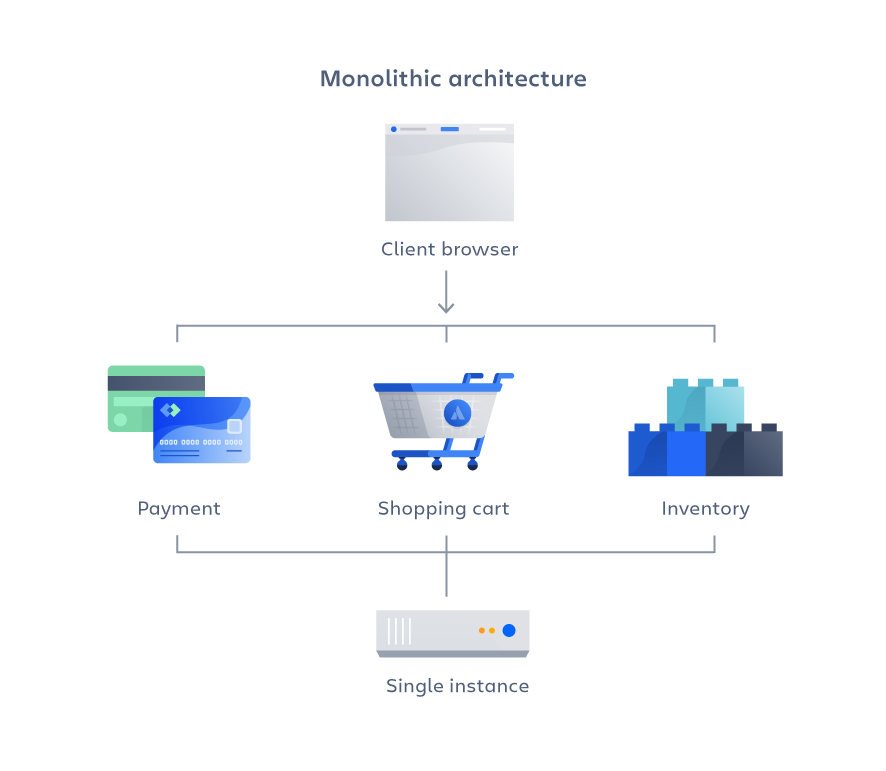
\includegraphics[width=\linewidth]{img/cap2/Monolithic_architecture.png}
		\end{subfigure}
		\begin{subfigure}{0.5\textwidth}
			\centering
			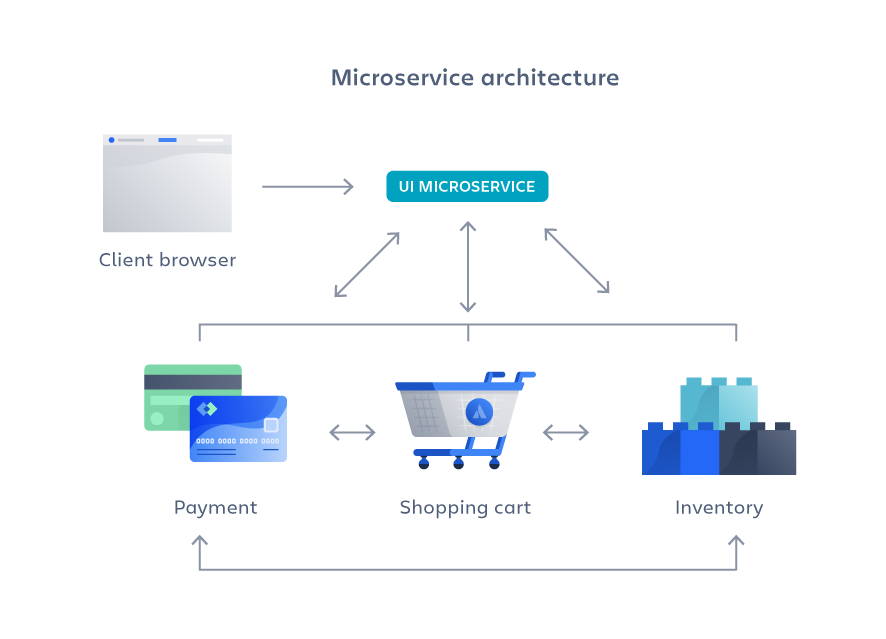
\includegraphics[width=\linewidth]{img/cap2/Microservice_architecture.png}
		\end{subfigure}
		\caption{Principio di funzionamento di un'applicazione monolitica e una a microservizi\cite{site:archComparison} }
	\end{figure}
	
	
	
\section{Deployment tradizionale}

	La metodologia tradizionale di deployment prevede l'esecuzione delle applicazioni direttamente sul server fisico.
	Sebbene semplice ed immediato questo modo di procedere non è ottimale, non permette infatti di scalare l'applicazione ponendo dei limiti sull'utilizzo di risorse (CPU, RAM, disco,\dots) e si corre il rischio che una seconda applicazione non riesca a garantire le prestazioni desiderate.
	Si potrebbe cercare un'alternativa a questo problema eseguendo ogni applicazione su un server fisico distinto, ma anche una tale soluzione non è adatta a un contesto reale risultando molto costosa e portando a un sottoutilizzo delle risorse complessive\cite{doc:kube}.



\section{Deployment su macchine virtuali}

	Le macchine virtuali sono pacchetti software piuttosto pesanti, in grado di eseguire l'emulazione dei dispositivi hardware di basso livello quali CPU, RAM, dischi e schede di rete.
	Il deployment su macchine virtuali (anche chiamato deployment virtualizzato) prevede l'esecuzione di più macchine virtuali sul server fisico, ciascuna delle quali esegue un sistema operativo che a sua volta esegue una o più applicazioni.
	Un simile approccio è in grado di far fronte ad alcune delle problematiche del deployment tradizionale:
	
	\begin{itemize}
		\item \emph{Limitazione delle risorse:}
			In funzione di quanto detto sopra è possibile limitare le risorse dedicate ad una macchina virtuale in termini di tempo di CPU, quantità di RAM, etc.
		\item \emph{Isolamento:}
			Le macchine virtuali vengono eseguite in un ambiente isolato e completamente autonomo che le rende immuni da tentativi di interferenza da parte di altre macchine virtuali attive sullo stesso host.
	\end{itemize}
	
	Contrariamente, i principali svantaggi delle macchine virtuali riguardano la ridotta velocità di generazione e distribuzione delle stesse e il maggiore spazio di archiviazione richiesto:
	trattandosi di \emph{immagini} di un sistema indipendente possono infatti richiedere diverso tempo per essere generate e configurate, l'affiancamento di diverse macchine virtuali porta inoltre alla duplicazione del sistema operativo installato su di esse, con un conseguente utilizzo di spazio di archiviazione.



\section{Deployment su container}
	
	\label{sec:depl_on_cont}
	Un \emph{container} è un modello di virtualizzazione più leggero rispetto ad una macchina virtuale che racchiude un software e tutte le dipendenze necessarie ad eseguirlo.
	Al pari delle macchine virtuali i container rappresentano un ambiente isolato, con risorse limitate ed un proprio file system per l'esecuzione del software ma non virtualizzano un intero sistema operativo.
	L'uso di container offre una grande efficienza in fase di sviluppo  e di esecuzione, contengono infatti solo software di alto livello e sono molto veloci da modificare, oltre al fatto che non dovendo virtualizzare un sistema operativo la loro esecuzione risulta molto più rapida e meno esosa di risorse hardware.
	Per finire molti sistemi runtime per container mettono a disposizione degli sviluppatori repository pubbliche con immagini preconfezionate di software popolari, il tutto al fine di avere uno sviluppo ancora più rapido
	\cite{doc:kube, site:container_vs_VM}.
	
	\begin{figure}[tbp]
		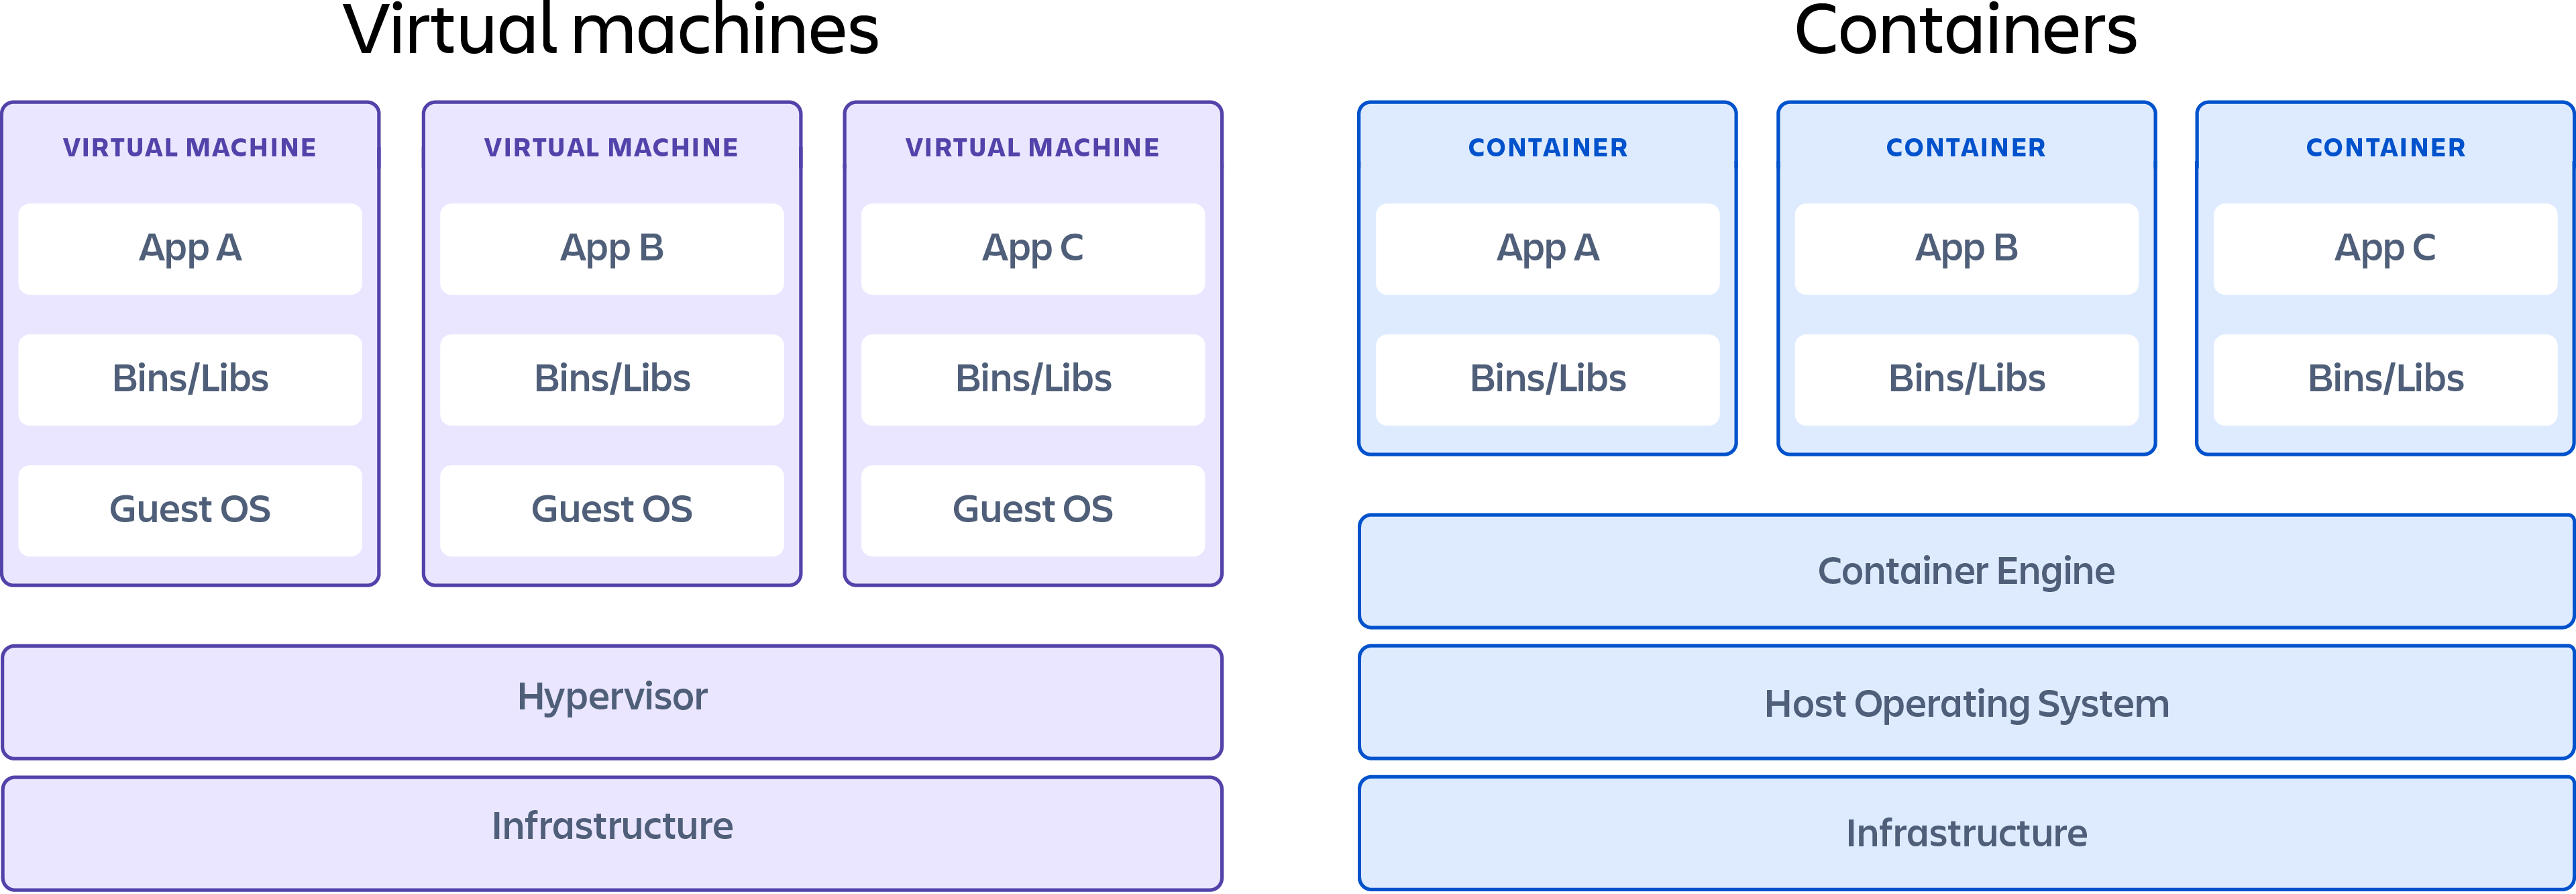
\includegraphics[width=\textwidth]{img/cap2/Diagram_Containers_VirtualMachines.png}
		\caption{Confronto tra un sistema basato su macchine virtuali e container\cite{site:container_vs_VM}}
		\label{fig:VM_vs_container}
	\end{figure}










